%%%%%%%%%%%%%%%%%%%%%%%%%%%%%%%%%%%%%%%%%%%%%%%%%%%%%%%%%%%%%%%%%%%%%%%%%%%%%%%
%  s03a-floer.tex —— §3 Floer 上同调（前半：§3.1–§3.5）
%  原文：Ivan Smith, A Symplectic Prolegomenon, arXiv:1401.0269v2
%  源码行：508–727（正文），对应原书第 8–18 页
%%%%%%%%%%%%%%%%%%%%%%%%%%%%%%%%%%%%%%%%%%%%%%%%%%%%%%%%%%%%%%%%%%%%%%%%%%%%%%%

\section{Floer 上同调}\label{Sec:Floer}

\begin{keypoints}
\begin{itemize}
  \item \textbf{核心图像}：$HF^*(L,L')$ 由计数以 $L,L'$ 为边界条件的全纯条带（等价地，带两个边界标记点的全纯圆盘）给出，是拉格朗日相交数的“范畴化”；$d^2=0$ 的机制与 Morse 理论同源——一维模空间的紧化边界恰好标号出 $d^2$ 的各项贡献。
  \item \textbf{关键工具}：Cauchy–Riemann 算子的椭圆性（横截性，Sard–Smale 定理）、Gromov 紧性、Maslov 分次，以及必要时改取 Novikov 域作系数。
  \item \textbf{核心障碍}：附着在条带边界上的圆盘泡会给一维模空间添出多余边界、破坏 $d^2=0$；回避之道有三条——先验排除泡（非球性/恰当性）、因维数理由排除泡（单调性）、以障碍理论消去泡（界定上链）。
  \item \textbf{代数结构与不变量}：三角乘积 $\mu^2$ 使 $HF^*(L,L)$ 成为（上同调）幺环，并有 Oh 谱序列 $H^*(L;\Lambda)\Rightarrow HF^*(L,L)$（Morse–Bott 或“pearl”模型）；$\mu^2$ 还组织出 Donaldson 范畴、正合三角（Lagrange 手术、Dehn 扭转）与 quilt 函子。
  \item \textbf{应用}：Hamilton 不可移开性、余切丛中 Arnol'd 猜想的一半，以及用 Floer 上同调的增长速率重述 Nielsen–Thurston 分类、证明 Dehn 扭转在 $\pi_0\Symp_{ct}(T^*S^n)$ 中的无限阶。
  \item \textbf{遗留问题}：仅有环结构不足以从一组“生成元”恢复一般对象的 Floer 上同调（§3.9）；正确的结构是 $A_\infty$-范畴，这正是 §4 的主题。
\end{itemize}
\end{keypoints}

\subsection{定义概述}

固定一个系数域 $\bK$。在适当的技术性假设下，Floer 上同调给一对闭的定向拉格朗日子流形 $L, L' \subset X$ 配置一个 $\bK$ 上的 $\bZ_2$-分次向量空间 $HF^*(L,L')$，它具有如下基本特征：
\begin{enumerate}
\item 欧拉示性数 $\chi(HF^*(L,L')) = (-1)^{n(n+1)/2}\, [L]\cdot[L']$ 还原出 $L, L'$ 所定义的同调类的代数相交数；
\item 有 Poincar\'e 对偶同构 $HF^*(L,L') \cong HF^{n-*}(L',L)^{\vee}$；
\item 空间 $HF^*(L,L')$ 在 $L$ 或 $L'$ 的 Hamilton 同痕下不变，即对任意 Hamilton 辛同胚 $\phi$ 有 $HF^*(L,L') \cong HF^*(\phi(L), L')$；
\item 当 $L$ 与 $L'$ 不相交时 $HF^*(L, L') = 0$；于是它的非零性给出 Hamilton 不可移开性的一个障碍。
\end{enumerate}

设 $L, L'$ 是辛流形 $(X,\omega)$ 的闭的可定向拉格朗日子流形。我们假设 $X$ 是闭的，或者“在无穷远处凸”，即存在 $X$ 上的驯服近复结构 $I$，以及一个穷竭（一列相对紧的开子集 $U_1 \subset U_2 \subset \cdots$，其并为 $X$），使得若 $S$ 是带非空边界的连通紧 Riemann 曲面、$u: S \rightarrow X$ 是 $I$-全纯映射且 $u(\partial S) \subset U_k$，则必有 $u(S) \subset U_{k+1}$。由 Stein 流形上的多重次调和穷竭函数得到的辛结构满足这些性质 \cite{CieliebakEliashberg}。

选取紧支的时间依赖 Hamilton 量 $H \in \smooth_{ct}([0,1] \times X,\bR)$，其相伴的 Hamilton 同痕 $(\phi^t)$ 具有性质：$\phi^1(L)$ 与 $L'$ 横截相交。若 char$(\bK) = 2$，则 Floer 上链复形按定义由该交点集在 $\bK$ 上自由生成。若 $\textrm{char}(\bK)\neq 2$，则指标理论给每个交点（即 Hamilton 弦）$x$ 配置一个 1 维 $\bK$-向量空间 $\mathrm{or}_x$，它由两个元素（$x$ 处的“相合定向”）生成，并满足两者之和为零这一关系。为定义微分，选取 $X$ 上一族一般的驯服近复结构 $J=\{J_t\}_{t\in[0,1]}$。给定两个交点 $x_\pm$，以 $\scrM(x_-,x_+)$ 记 Floer 轨道的模空间
\begin{equation} \label{eq:Floer}
\begin{aligned}
 & u: \bR \times [0,1] \longrightarrow X, \\
 & u(s,0) \in L, \;\; u(s,1) \in L', \\
 & \partial_s u + J(t,u) \big(\partial_tu - X(t,u)\big) = 0, \\
 & \textstyle\lim_{s \rightarrow \pm\infty} u(s,t) = y_\pm(t), \\
 & E(u) = \int u^*\omega = \int \!\!\! \int \big| \partial u / \partial s \big|^2 \, ds\,dt \ < \infty,
\end{aligned}
\end{equation}
其中 $X$ 表示 $H$ 的 Hamilton 向量场，即 $\omega(X,\cdot) = dH$，而 $y_\pm$ 是 $X$ 的流线，满足 $y_\pm(1) = x_\pm$。于是
\begin{equation} \label{Eqn:FloerDifferential}
d_J(x_+) = \sum_{x_-} n_{x_+, x_-} x_-
\end{equation} 其中 $n_{x_+, x_-} \in \bK$ 计数孤立解 $u \in \scrM(x_-, x_+) / \bR$（$\bR$-作用由 $s$ 方向的平移给出），其符号被典范地编码为一个同构 $\delta_u: \mathrm{or}_{x_+} \stackrel{\cong}{\longrightarrow} \mathrm{or}_{x_-}$。人们常常按相应全纯圆盘的辛面积对解加权计数；关于这一点以及 \eqref{Eqn:FloerDifferential} 的收敛性问题，见第 \ref{Sec:Novikov} 节。

\begin{figure}[ht]
  \centering
  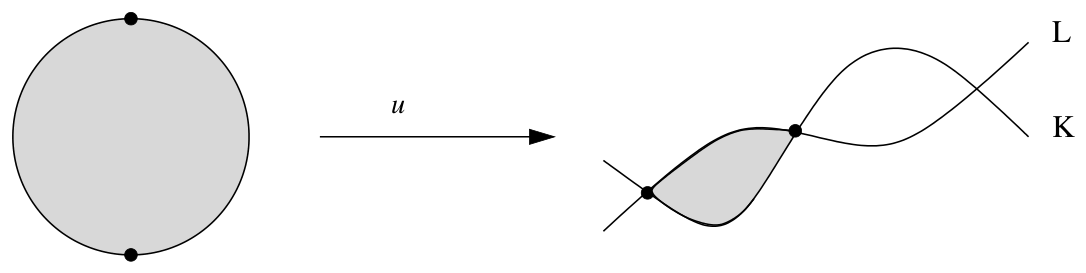
\includegraphics[width=0.55\textwidth]{fig01-floer-whitney.png}
  \caption{Floer 微分（即 $CF^*(L,K)$ 上的微分；原文 Figure~1，第 8 页）。\label{Fig:FloerWhitney}}
\end{figure}

设 $L \pitchfork L'$ 横截，并取 $H \equiv 0$。则方程 \eqref{eq:Floer} 就是通常的 Cauchy–Riemann 方程 $\cdbar_J(u) = 0$。存在共形等同 $\bR\times[0,1] \cong D^2 \backslash \{\pm i\}$，而 Floer 方程的解可延拓为闭圆盘上的连续映射，把 $\pm i$ 送到所选交点 $x_{\pm} \in L \cap L'$；在这个意义上，Floer 微分计数的是全纯圆盘，见图 \ref{Fig:FloerWhitney}。关键在于：(i) 对一般的数据，应当预期 \eqref{eq:Floer} 的解模空间是有限维光滑流形；(ii) 这些模空间具有几何上有意义的紧化。模空间的光滑性与有限维性是 Cauchy–Riemann 方程（带全实边界条件）椭圆性的推论；而面积一致有界的曲线空间之紧化的几何描述，则是 Deligne 与 Mumford 引入稳定曲线模空间那一思路的变体：边界层用带结点的 Riemann 曲面（圆盘与球面构成的树）来标号。

这是一个非平凡的定理（需要下面第 \ref{Sec:GeometricHyp} 节讨论的附加假设）：$d_J^2 = 0$，因此这确实定义了一个链复形。与 Morse 理论一样，$d_J^2=0$ 背后的机制是：\eqref{eq:Floer} 解的 1 维模空间具有紧化，其边界层标号出 $d_J^2$ 的各项贡献；而附加假设排除掉其他会打乱这种标号的不受欢迎的退化。
% [Tutor Note: $d_J^2=0$ 的证明不在正文，其要点是对（模去平移的）1 维解模空间做 Gromov 紧化：
%   边界层要么在角点处破裂、给出 $d_J\circ d_J$ 的各项，要么冒出圆盘泡/球面泡；只有排除后者，边界恒等式才恰好给出 $d_J^2=0$。
%   注意 $E(u) < \infty$ 这一条是紧化的定量前提，不能省略。]
在此前提下，相应的上同调 $HF^*(L,L')$ 就称为 Floer 上同调。一个“选择的同伦”论证说明它既不依赖 $J$ 的选取，也不依赖 $L$ 或 $L'$ 的 Hamilton 同痕。事实上，给定一族近复结构 $\{J_s\}$ 或一个在 $|s| \gg 0$ 时恒定的运动拉格朗日边界条件 $\{L_s\}$，人们考虑连续映射方程
\begin{equation} \label{Eqn:Continuation}
 \partial_s u + J_{s}(t,u) \big(\partial_tu - X_{s}(t,u)\big) = 0
\end{equation}  
其边界条件为 $\{L_s, L'\}$，解的数量给出相关 Floer 复形之间的链映射。把该映射与由逆同伦诱导的映射的复合形变回常值族，便可看出它在同调上诱导同构，而常值族诱导上同调上的恒等。

\begin{Example}
令 $X=T^*S^1$，考虑由 0-截面与一个同伦的圆给出的拉格朗日 $L, L'$，后者与该截面横截相交于两点 $a,b$。有两个跨接两圆的月牙形区域 $u,v$，由 Riemann 映射定理，它们共形地是全纯条带的像。复形 $CF(L, L') = \bK\langle a\rangle \oplus \bK\langle b\rangle$。取 $\bK = \bC$。按面积 $e^{-\int_u \omega}$ 对全纯条带 $u$ 加权计数，并计入全纯条带的定向，可得
\[
\partial(a) = (e^{-\omega(u)} - e^{-\omega(v)}) \, b, \qquad \partial(b) = 0.
\]
因此，除非 $\omega(u) = \omega(v)$，否则 $HF(L,L') =0$；确实，若面积不同，可以把 $L'$ Hamilton 同痕为一个与 $L$ 平行、与 $L$ 不交的平移。若两月牙形面积相等，则 $L'$ 是 $L$ 的 Hamilton 像，且 $HF(L,L')$ 的秩为 2。
\end{Example}

Floer 理论中的一篇典型论文总是先对环境几何给出一系列技术性假设。在第 \ref{Sec:GeometricHyp} 与第 \ref{Sec:AlgebraicHyp} 节中，我们汇集其中最常见的一些，指出它们各自在何处起作用，以及在其不成立或成立时人们能得到什么。

\subsection{定义的动机} 下面第一个动机在历史上是准确的，其余几个则提供了有用的背景。

\subsubsection{路径空间上的 Morse 理论} 设 $Q$ 是光滑有限维流形，$f: Q \rightarrow \bR$ 是一般函数（特别地，其临界点非退化），则 $f$ 的 Morse 复形 $C^*(f)$ 由 $f$ 的临界点生成，其微分计数梯度流线
\[
\gamma: \bR \rightarrow Q,  \quad \dot{\gamma}(t) = \nabla f_{\gamma(t)}
\]
其中梯度流是相对于 $Q$ 上某个辅助选取的 Riemann 度量而言的。有一个由 Novikov 给出的推广：把函数 $f$ 换成一个不一定恰当的一形式。Floer 复形正是该构造的形式类比：把 $Q$ 换成路径空间 $\mathcal{P}(L,L')$，把函数 $f$ 换成作用泛函（一形式）$\scrA$——它沿某条路径 $\gamma$ 的无穷小变分 $\xi$ 积分辛形式，即 $\xi \mapsto \int_0^1\omega(\xi, \dot{\gamma}) dt$，其中 $\xi$ 是沿 $\gamma$ 的向量场。$\scrA$ 的临界点是常值路径，也就是交点。固定 $(X,\omega)$ 上一个相容的近复结构 $J$，即 $J$ 驯服且 $\omega(J\cdot, J\cdot) = \omega(\cdot,\cdot)$。于是 $J$ 在路径空间上定义了一个 $L^2$-度量，而形式的梯度流方程恰是 $H=0$ 时的 Cauchy–Riemann 方程 \eqref{eq:Floer}。

\begin{Remark} \label{Rem:Filtration}
$HF^*(L,L')$ 的梯度流观点还揭示出额外的结构：若 $\scrA$ 是单值的，则复形 $CF^*(L,L')$ 自然被作用量（即泛函 $\scrA$ 的取值）滤过，而 Floer 微分保持该滤过。
% [Tutor Note: 这里“单值”是关键：作用量泛函一般只在覆叠空间上良定义，若辛形式在 $\pi_2(X,L)$ 上不零化，
%   则 $\scrA$ 多值，按作用量滤过只能在万有覆叠上谈；这正是后文要引入 Novikov 系数的原因之一。]
\end{Remark}

\subsubsection{几何相交数} 设 $\Sigma_g$ 是亏格为 $g$ 的定向曲面。对 $\Sigma$ 上（同伦非平凡的）曲线 $\alpha, \beta$，以 $\iota(\alpha,\beta) \in \bZ_{\geq 0}$ 记其几何相交数。一个微分同胚 $f$ 给出序列 $\iota(\alpha, f^n(\beta))$（$n\in \bN$），它只依赖 $f$ 的映射类 $[f] \in \pi_0\Diff(\Sigma)$。Nielsen–Thurston 分类可以用动力学的语言表述如下 \cite{FLP}：每个 $f$ 满足下列之一。

\begin{itemize}
\item $f$ 是可约的：若 $f$ 的某个幂保持一条简单闭曲线（同痕意义下）；
\item $f$ 是周期的：若对任意 $\alpha, \beta$，序列 $\{\iota(\alpha, f^n\beta)\}$ 关于 $n$ 是周期的；
\item $f$ 是伪 Anosov 的：若对任意 $\alpha,\beta$，序列 $\{\iota(\alpha, f^n\beta)\}$ 关于 $n$ 指数增长。
\end{itemize}

该分类应视为对曲面复杂度的归纳：可约情形表明 $f$（的某个幂）由某个更简单曲面的微分同胚诱导。在最有趣的伪 Anosov 情形，几何相交数增长率之对数与 $\alpha,\beta$ 无关，并且可由映射类 $f$ 在 Teichm\"uller 空间上作用的 Teichm\"uller 度量平移长度实现。$\Sigma$ 的任意微分同胚都同痕于一个保面积微分同胚。对不互相同伦（也不同伦平凡）的曲线 $\alpha, \beta$，有 $\iota(\alpha,\beta) = \mathrm{rk}\, HF(\alpha,\beta)$，所以 Thurston 分类同时也是用 Floer 上同调增长率对辛映射类作出的分类。在高维寻找类似物是一个长期挑战。

\subsubsection{手术理论} 高维流形的分类依赖 Whitney 技巧。考虑单连通定向流形 $M$ 中两个互补维数的可定向子流形 $K^k, N^{d-k} \subset M^d$，其中 $d>4$、$k>2$。设 $K,N$ 交于一对相交符号相反的点 $\{x,y\}$；在 $K$ 与 $N$ 中分别取连接 $x$ 与 $y$ 的弧，Whitney 技巧便让 $K$ 沿一张跨接这两条弧的圆盘滑动（该圆盘由 $M$ 的单连通性保证存在；由于 $d > 4$ 且 $k>2$，可假定它嵌入且内部与 $K,N$ 不交），从而降低子流形的几何相交数。Floer 上同调设想的是 Whitney 技巧的一个精细版本：只允许通过沿\emph{全纯} Whitney 圆盘滑动来消去拉格朗日子流形之间多余的相交。

Floer 上同调自身的手术论方面尚待发展，即：给定一对恰交于两点并界定唯一全纯圆盘的拉格朗日子流形 $L, L'$，何时能通过 Hamilton 同痕移动 $L$ 来消去这两个交点，目前未知。这是该理论最基本的空白之一。

\subsubsection{量子上同调} Floer 上同调是闭弦不变量（通过对有理曲线的计数来定义）的开弦类比（涉及带边界的亏格零 Riemann 曲面）。闭辛流形 $X$ 的量子上同调作为加群是 $H^*(X;\bK)$（$\bK$ 通常是 Novikov 域，参看 \eqref{Eqn:NovikovField}），但它带有乘法 $\ast$，该乘法用 3 点 Gromov–Witten 不变量决定的高阶贡献来形变经典的相交积。对光滑射影簇，它可以纯代数几何地定义，即通过稳定映射模叠上的相交理论。若 $\phi: X\rightarrow X$ 是辛同胚，则对角线 $\Delta_X$ 与 $\phi$ 的图像 $\Gamma_{\phi}$ 都是 $(X,\omega) \times (X,-\omega)$ 中的拉格朗日，于是定义\footnote{$HF^*(\phi)$ 有一个更初等、适用范围更广的直接构造；但为简洁起见，我们满足于通过拉格朗日 Floer 上同调来描述。} $CF^*(\phi) = CF^*(\Delta_X, \Gamma_{\phi})$。$CF^*(\phi)$ 的生成元由 $\phi$ 的不动点给出（假定这些不动点非退化）。为把两种讨论联系起来：有同构 $HF^*(\id) \cong QH^*(X)$。

量子上同调本身就是一个重要的不变量：它区分出若干有趣的辛流形集合（例如证明辛结构模微分同胚的模空间在 $K \times S^2$ 上有无穷多个分支，其中 $K \subset \bC\bP^3$ 是四次 $K3$ 曲面）；它在三维 flop 下不变；且与可积系统有深刻联系。若把 $QH^*(X) \cong HF^*(\Delta_X, \Delta_X)$ 视为一种影响深远的推广，那么一般拉格朗日对之间的 Floer 上同调的缺点在于：它很少能用代数几何方法计算——至少在镜像对称带来洞见之前如此。

\subsection{定义的技术细节：几何假设\label{Sec:GeometricHyp}}

低维拓扑与几何中的许多不变量都是通过计数某个椭圆偏微分方程的解来定义的。这样的定义预设：在好的情形下，模空间是紧的零维流形，因而计数才有意义。问题的核心于是归结为克服横截性（使解空间成为已知维数的流形）与紧性（使零维解空间成为有限集）这两方面的困难。

\subsubsection{横截性.} $X$ 上的驯服近复结构 $J$ 称为对某个特定的模问题\emph{正则}的（例如对映射 $u: \bP^1 \rightarrow X$，或对代表固定相对同调类、满足 $\cdbar_J(u) = 0$ 的圆盘 $u: (D^2,\partial D^2) \rightarrow (X,L)$），若 Cauchy–Riemann 方程或 Floer 方程的线性化 $D_u = D(\cdbar_J)_u$ 在每个解 $u$ 处都满射。在这种情形，Sard–Smale 隐函数定理表明解 $u$ 的模空间局部是光滑流形，其维数等于算子 $D_u$ 的指标。Sard–Smale 定理涉及 Banach 流形之间的映射，因此有一个常规的麻烦：应先把 $\cdbar$-算子延拓为 Banach 丛 $\cdbar_J: L^{k,p}(\Sigma, X) \rightarrow L^{k-1,p}(\mathcal{E})$ 的一个截面（其中 $\mathcal{E}_u = \Omega^{0,1}(u^*TX)$），定义在 $L^{k,p}$ 映射空间上（若 $kp>2$ 则映射连续，逐点边界条件才有意义），从而对正则的 $J$ 得到光滑的解模空间——它\emph{先验地}由低正则性的映射组成；然后再用“自举（bootstrapping）”推出方程的任一 $L^{k,p}$-解其实都是光滑映射。
% [Tutor Note: Sard–Smale 只适用于可分 Banach 流形之间的 Fredholm 截面，所以必须先做 $L^{k,p}$ 完备化；
%   把“解”直接当成 $C^\infty$ 映射来谈横截性是常见的形式错误。椭圆正则性负责把 $L^{k,p}$ 解提升回光滑解。]

达到“你想要的那么多横截性”存在内在障碍。例如设 $X$ 是闭辛 6-流形且 $c_1(X) =0$。对任意 $A \in H_2(X;\bZ)$，类 $A$ 中无参数有理曲线的虚拟维数为 $0$。然而，若 $u: \bP^1 \rightarrow X$ 代表类 $A$，则类 $kA$ 可由映射 $\bP^1 \stackrel{k:1}{\longrightarrow} \bP^1 \stackrel{u}{\longrightarrow} X$ 代表，于是类 $kA$ 中曲线的模空间至少和 $\bP^1$ 到自身的 $k$ 次覆盖的 Hurwitz 空间一样大，不可能维数为零。这说明：若不扰动 Floer 方程或 Cauchy–Riemann 方程本身以破坏覆盖的对称性（例如让近复结构 $J$ 依赖曲线的定义域上的点，从而不具任何有限对称性），就不能指望在多重覆盖曲线上达到横截性。对有理曲线，一般选取的 $J$ 对单重（非多重覆盖）曲线是正则的。对圆盘，若视其为条带 $D^2 \backslash \{\pm 1\}$ 上在边界穿孔处光滑延拓的映射，则一族一般的复结构 $\{J_t\}_{t\in[0,1]}$ 对具有内射点 $x$（即满足 $u^{-1}(u(x)) = \{x\}$ 的点）的解仍是正则的。

\begin{Example} \label{Ex:TransversalityFiniteGroup} 还有与多重覆盖无关的横截性问题。设 $X$ 带有一个辛对合 $\iota$，其不动点集为 $X^{\iota}$，并设有 $\iota$-不变的拉格朗日 $L_i$，满足 $L_i^{\iota} = L_i \cap X^{\iota}$ 是 $X^{\iota}$ 中的拉格朗日。若对 $x,y \in L_1^{\iota} \cap L_2^{\iota}$，含于 $X^{\iota}$ 内的 Floer 轨道 $u$ 所在模空间的虚拟维数大于 $u$ 在 $X$ 中相应的虚拟维数，则不能同时要求该曲线在两个空间中都正则：正则 $J$ 的稠密集可能与 $\iota$-不变 $J$ 的无限余维轨迹不相交。（若不动点集中没有轨道，则\emph{可以}实现等变横截性 \cite{Khovanov-Seidel}。）
% [Tutor Note: 等变横截性失败的机制值得记住：正则 $J$ 是稠开集，而 $\iota$-不变 $J$ 是无限余维的闭子集，二者可能不交。
%   因此不能“先取一般 $J$ 再对称化”；正确做法是在等变范畴内单独做横截性论证（如固定轨迹内无轨道时）。]
\end{Example}

\subsubsection{通过冒泡的紧性.} 解模空间即使正则，通常也不紧。Gromov 紧性 \cite{Gromov} 给出一个紧化，其中包含带结点的曲线（球面与圆盘构成的树）。一个要点是：虽然 Floer 方程是 Cauchy–Riemann 方程的形变版本，泡却来自重新尺度化过程，这意味着它们满足未形变的方程 $\overline{\partial}_J(u) = 0$。因此，一般不能指望通过一般地选取非齐次项或依赖定义域的近复结构来克服多重覆盖泡带来的横截性问题。通常，全纯曲线紧化空间的边界层维数可能远大于人们想要紧化的开层维数。对此没有容易的一般性解决办法（已有的解法 \cite{FO3:technical, HWZ} 是在映射的 Banach 空间内扰动解模空间，而不是扰动方程或其他几何数据本身，统称为\emph{虚拟扰动理论}）。

具体地说，要定义 Floer 上同调，需要知道 Floer 复形中 $d^2 = 0$。与 Morse 理论一样，这一关系的证明来自研究（模去平移的）1 维解模空间的边界。除了对 $d^2$ 有贡献的边界层之外，还有一种有问题的破裂：一个以 $L$ 或 $L'$ 为边界的全纯圆盘从中冒出，见图 \ref{Fig:Bubble}。（圆盘的边界值被一个常值映射送到拉格朗日上、从而给出 $X$ 中经过 $L$ 的有理曲线这一退化情形，同样有问题。）

\begin{figure}[ht]
  \centering
  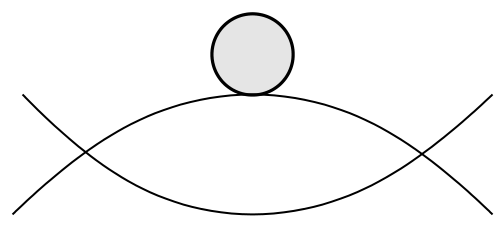
\includegraphics[width=0.4\textwidth]{fig02-disc-bubble.png}
  \caption{全纯圆盘泡会阻碍 Floer 复形中的 $d^2 = 0$（原文 Figure~2，第 12 页）。\label{Fig:Bubble}}
\end{figure}

有三种基本路线可以回避圆盘冒泡带来的问题。
% [Tutor Note: 三条路线不要混为一谈：(i) 非球性/恰当性——面积上根本不容许泡存在；
%   (ii) 单调性——允许泡，但按虚拟维数它扫出的链在 $L$ 中是边界，故对 $d^2$ 无贡献；
%   (iii) 障碍理论——允许泡贡献，用界定上链把这些边界“配平”。恰当性蕴含非球性，但反之不然。]

\subsubsection{先验地排除泡：非球性或恰当性.\label{Sec:exact}} 这里要求对所考虑的一切拉格朗日都有 $\langle \omega, \pi_2(X,L)\rangle = 0$（这特别蕴含 $X$ 中没有辛 2-球面）。由于泡是全纯的，若非常值，其面积必严格为正，这由基本恒等式
\[
\int_C u^*\omega \ = \ \int_C \| du\|_J^2
\] 
对带拉格朗日边界、$J$ 与 $\omega$ 相容的 $J$-全纯曲线 $u: C \rightarrow X$ 成立。这是本学科最早几篇论文（尤其是 Floer 本人的工作）所采用的设定。

对非紧辛流形 $X$，若辛形式 $\omega = d\theta$ 整体恰当，且拉格朗日 $L\subset X$ 是恰当的（即 $\theta|_L = df$ 在 $H^1(L)$ 中为零），则由 Stokes 定理立即排除泡。（然而 $\omega^n > 0$ 表明 $\omega$ 的恰当性与 $X$ 为闭流形不相容。）$X$ 的非紧性引入模空间失去紧性的另一个可能来源：解可能逃逸到无穷远；这由另一套机制控制，通常是某种极值原理的变体，它要求对无穷远处的几何加以控制。Stein 流形 $X$（特别是仿射簇）在无穷远处以接触锥为模型，即紧集之外它们辛同胚于 $(Y\times \bR_+, d(e^t\alpha))$ 的某个子集，其中 $(Y,\alpha)$ 是接触的、$t\in\bR_+$。对全纯曲线 $u: \Sigma \rightarrow X$，（部分定义的）函数 $t\circ u$ 是次调和的，$\Delta(t\circ u) \geq 0$，这意味着该函数没有内部最大值。由此推出：边界包含在内部 $X \backslash (X \cap Y\times\bR_+)$ 中的全纯曲线完全含于内部，因此 Stein 流形在前文所述意义下在无穷远处凸。

一个可追溯到 Floer 的论证，把 $L, \phi_H^t(L)$（其中 $\phi_H^t$ 是 $L$ 上某个 Morse 函数 $H$ 的小时间流，$J$ 是仔细选取的时间依赖近复结构）之间的、保持在 $L$ 附近的全纯条带，与 $H$ 的梯度流线等同起来。因此作为向量空间可以认同 $CF^*(L,L) = C^*_{Morse}(L)$。在不存在以 $L$ 为边界的全纯圆盘时，紧性论证表明没有其他能对 Floer 微分有贡献的全纯条带，从而：

\begin{Theorem}[Floer] \label{Lem:Floer}
若 $\langle \omega, \pi_2(X,L) \rangle = 0$，则 $HF^*(L,L) \cong H^*(L)$。
\end{Theorem}

这恢复了 Gromov 的定理 \cite{Gromov}：$\bC^n$ 不含闭的恰当拉格朗日——因为这样的 $L$ 可被移开，从而 $HF(L,L)=0$。（恰当拉格朗日 $L_t$ 的任何同痕 $\{L_t\} \subset X$ 都由 $X$ 的 Hamilton 流诱导；特别地，恰当同痕不改变 Floer 上同调。）

\subsubsection{因维数理由排除泡：单调性.\label{Sec:Monotone}} 若可能的圆盘泡与球面泡所扫出的 $X$ 的子集具有足够高的（余）维数，则对 Floer 方程中数据的\emph{一般}选取（近复结构、Hamilton 项），1 维模空间中出现的全纯条带的边界值永远不会与泡相交。这一解决办法的典型情形是 $X$ 与 $L$ 都\emph{单调}，即 Maslov 指标 $\mu_L$ 与面积同态在 $\pi_2(X,L)$ 上正比例；特别地，$\omega_X$ 与 $c_1(X)$ 在 $\pi_2(X)$ 上正比例，这是代数几何中 Fano 条件的辛类比。$\bP^n$ 中总次数 $\leq n$ 足够低的超曲面或完全交是单调的。单调辛流形的极小 Chern 数 $N_{min}(X)>0$ 由等式 $\{\langle c_1(X), \pi_2(X)\rangle\} = N_{min}(X)\bZ$ 定义。类似地，单调拉格朗日 $L\subset X$ 有极小 Maslov 数 $N_{min}(L)>0$。由于在 $H^2(X,L)\rightarrow H^2(X)$ 之下 $\mu_L \mapsto 2c_1(X)$，当 $\pi_1(L)=0$ 时 $N_{min}(L) = 2N_{min}(X)$。
% [Tutor Note: $\mu_L \mapsto 2c_1(X)$ 中的因子 2 来自 Maslov 指标与 Chern 数的换算（圆盘边界绕行时切空间转两圈）。
%   由此 $N_{min}(L)=2N_{min}(X)$（当 $\pi_1(L)=0$）；核对 $\frak{m}_0$ 与单调性假设时，此处最容易差一个因子 2。]

先设 $X$ 单调且 $N_{min}(X) \geq 2$，而 $K, L\subset X$ 是单调拉格朗日，各自 $N_{min}\geq 4$。图 \ref{Fig:Bubble} 所描绘的构型，形式上是一个纤维积 $\scrM_{bubble} \times_L \scrM_{Floer}$：Floer 条带空间与圆盘泡空间的纤维积，沿（假定光滑且横截的）到 $L$ 的赋值映射取。某个类 $\beta$ 中 $L$ 上无参数圆盘的模空间的虚拟维数为 $n+\mu_L(\beta)-3 \geq n+1$，故赋值后在 $L$ 上作为链是平凡的，即它们是 $C^*_{sing}(L)$ 中的边界。这意味着在代数上，计算 $CF^*(K,L)$ 中的 $d^2$ 时不会出现带圆盘泡的退化。

在极小 Maslov 指标为 2 的单调拉格朗日这一特殊情形，有一点细微却重要的差别：Maslov 2 圆盘的模空间是 $(n-1)$ 维的，在边界标记点处赋值后，类 $\beta$ 的圆盘以某个重数 $n_{\beta}$ 扫出 $L$。这引出一个特殊的“障碍项”
\[
\frak{m}_0(L) = \sum_{\beta} n_{\beta} q^{\langle \omega, \beta\rangle} \in \bC[\![q]\!].
\] 对满足 $\frak{m}_0(L) = \frak{m}_0(L')$ 的拉格朗日对 $L, L'$，仍可定义 Floer 上同调，因为此时相关的额外边界可以互相抵消；但对 $\frak{m}_0$ 值不同的单调拉格朗日，Floer 复形中\emph{不}成立 $d^2=0$。

\begin{Example} \label{Ex:CY} 若 $X$ 是 Calabi–Yau 曲面，则 Maslov 零的拉格朗日的圆盘泡虚拟维数为负：$n+\mu-3 = -1$，故对一般的 $J$ 没有泡，可以把 $CF^*(L,L)$ 定义为上链复形。然而，在拉格朗日的一参数族中可能出现孤立的圆盘泡，这意味着所得的 Floer 上同调\emph{先验地}不清楚是否 Hamilton 不变：连续映射方程 \eqref{Eqn:Continuation} 可能因冒泡而不是链映射。参看 \cite[Section 8]{Seidel:HMSquartic}。
% [Tutor Note: 虚拟维数为负只保证“一般 $J$ 下没有泡”，不保证一族 $J_t$ 或一族 $L_t$ 中没有孤立泡；
%   这正是“$HF$ 定义出来了、却未必 Hamilton 不变”的典型陷阱，需要额外论证连续映射是链映射。]
\end{Example}

\subsubsection{消去泡：障碍理论} 若圆盘泡出现，它们会给 1 维模空间添上多余的边界，使 $d^2=0$ 不成立。若能“手工”抵消这些多余边界，便可挽救局面：在图 \ref{Fig:Bubble} 中，赋值像 $ev(\scrM_{bubble}) \in C^*_{sing}(L)$ 可能是边界，尽管并非因维数理由而平凡地是边界。这正是 Floer 上同调的\emph{障碍理论}的起源。它并不总是适用（圆盘泡边界扫出的 $L$ 中轨迹可能不是零调的），适用时又依赖于界定上链的额外选取（这使 Hamilton 不变性变得复杂，参看例 \ref{Ex:CY}），但它提供了 Floer 理论迄今得以发展的最一般框架，尤其是 \cite{FO3, FO3:technical}。这一策略奏效的情形类足够宽广，比起其他几种是相当大的进展，但这项工作的细节——一般要依赖虚拟扰动理论——颇为可畏。

为照顾一般情形，Floer 上同调有良好定义的拉格朗日被称为\emph{无障碍的}。

\subsection{定义的技术细节：代数假设\label{Sec:AlgebraicHyp}} 即使已经决定了允许哪一类拉格朗日子流形，它们所携带的附加结构仍有种种变化（这些结构的存在性可能施加进一步的限制）。

\subsubsection{系数环的选取.\label{Sec:Novikov}}

Gromov 紧性在有统一面积界时可控制全纯曲线序列的极限；但——正如 Novikov 的圆周值 Morse 理论——一个问题中仍可能遇到无穷多个模空间（此处是一对固定交点之间的连接条带）。若出现无穷多个模空间，为使和式 \eqref{Eqn:FloerDifferential} 有意义，就需要追踪同伦类。于是，$HF^*$ 最一般适用的定义要在 Novikov 域
\begin{equation} \label{Eqn:NovikovField}
\Lambda \ = \ \left\{ \sum a_i q^{\lambda_i} \ | \ a_i \in \bK, \lambda_i \in \bR, \lambda_i \rightarrow \infty \right\}
\end{equation}
上工作，其底层系数域为 $\bK$（若 $\bK$ 代数闭，则 $\Lambda$ 也代数闭）。然后定义 Floer 微分 \eqref{Eqn:FloerDifferential} 为
\begin{equation} \label{Eqn:FloerDifferential-Novikov}
d_J(x_+) = \sum_{\beta, x_-} n^{\beta}_{x_+, x_-} q^{\langle \omega, \beta\rangle} x_-
\end{equation}
其中 $\beta$ 是连接双边形的同伦类。有一个子环 $\Lambda_+ \subset \Lambda$，由最低 $q$ 幂次 $\geq 0$ 的幂级数组成。Floer 上同调只有在 Novikov 域上工作时才对 Hamilton 同痕不变；尽管如此，它在 $\Lambda_+$ 上仍承载非平凡信息。有限生成 $\Lambda_+$-模的分类定理表明
\[
HF(L,L') \cong \Lambda_+^r \, \bigoplus \ \oplus_{i=1}^n \Lambda_+ / \langle q^{k_i} \rangle
\]
挠部分在过渡到 $\Lambda$ 时显然消失，而自由加项保留下来；另一方面，显式的 Hamilton 同痕只能把系数 $k_i$ 改变不超过该同痕的 Hofer 范数——这是转到 Novikov 域上工作时丢失的信息。这一点在圆 $S^1 \subset \bC$ 这一最平凡的情形就已显现。该圆是 Hamilton 可移开的，故在 $\Lambda$ 上其自 Floer 上同调消失；而在环 $\Lambda_+$ 上自 Floer 上同调是挠群 $\Lambda_+ / \langle q^A \rangle$，其中 $A$ 是该圆所围的面积。于是，$\Lambda_+$ 上的 Floer 上同调记住了（在此情形下是初等的）事实：任何移开它的 Hamilton 量至少要用能量 $A$。
% [Tutor Note: $\Lambda$ 与 $\Lambda_+$ 的取舍是实用分水岭：只有 $\Lambda$ 上才有 Hamilton 同痕不变性；
%   而 $\Lambda_+$ 保留了 Hofer 范数能探测的能量下界（圆 $S^1\subset\bC$ 是最清楚的例子）。
%   另注意 $\Lambda$ 的指数满足 $\lambda_i \to +\infty$（形式幂级数），方向与通常 Laurent 级数相反。]

\begin{Example}
若 $L, L'$ 恰当，$\theta|_L = df$、$\theta|_{L'} = df'$，则交点 $x,y \in L\pitchfork L'$ 之间任一连通全纯条带的面积由 $f(x)-f'(y)$ 给出。统一的面积界与 Gromov 紧性蕴含只有有限多个同伦类 $\beta$ 能由全纯条带实现，因此和式 \eqref{Eqn:FloerDifferential} 是有限的。
\end{Example}

\subsubsection{Spin 结构与扭曲理论}

至此我们尚未提及域 $\bK$ 的特征。若它不等于 2，则 \eqref{Eqn:FloerDifferential} 或 \eqref{Eqn:FloerDifferential-Novikov} 中的计数必须是 0 维模空间的\emph{带符号}计数，因此这些模空间应当可定向。一个基本事实 \cite{deSilva,FO3} 是：$L$ 上 $Spin$ 结构的一个选取\footnote{用 $Pin$ 结构也够，但我们坚持用 $Spin$。}诱导出某个类 $\beta$ 中 $L$ 上全纯圆盘模空间 $\scrM(\beta)$ 的一个定向；环路 $\gamma: S^1 \rightarrow \scrM(\beta)$ 通过取边界值诱导映射 $\Gamma_{\gamma}: T^2 \rightarrow L$，且 $\langle w_1(\scrM(\beta)), \gamma\rangle = \langle w_2(L), \Gamma_{\gamma}\rangle$。同理，若 $L$ 不是 $Spin$ 的，就不能指望圆盘或 Floer 轨道的模空间可定向，此时应在特征 2 下工作。

拉格朗日上 $Spin$ 结构的存在意味着模空间具有定向。然而这些定向仍非典范的：人们可以用任一全纯圆盘与 $X$ 中某个与拉格朗日不交的余维 2 闭链的相交数，来扭转该圆盘计入 Floer 微分的符号；这种扭转与曲线的破裂以及由此定义 Floer 上同调（及其上以后会遇到的各种运算）的模空间紧化相容。结论是：实际上对任意“背景”类 $\beta \in H^2(X;\bZ_2)$ 的选择，都有一个版本的 Floer 上同调 $HF^*(L,L';\beta)$，其中拉格朗日应在“相对 spin”的意义下满足 $w_2(L) + \beta|_L = 0$。

\subsubsection{分次} 与经典代数拓扑的链复形不同，Floer 复形一般不是 $\bZ$-分次的。至少当拉格朗日子流形 $L, L'$ 定向时，横截交点有正负之分，这在复形上诱导一个 $\bZ_2$-分次（若拉格朗日可定向但未定向，这仍作为相对 $\bZ_2$-分次保留下来）。这可以细化为 $\bZ/N$ 分次，其中 $N$ 是拉格朗日的极小 Maslov 数。特别地，若 $L$ 与 $L'$ 的 Maslov 类为零（这尤其要求 $2c_1(X)=0$），则 Floer 复形可以 $\bZ$-分次。
% [Tutor Note: 分次有三个层次，切勿混用：$\bZ_2$（来自定向）$\subseteq$ $\bZ/N$（$N$ 为极小 Maslov 数）$\subseteq$ $\bZ$（Maslov 类为零，需 $2c_1(X)=0$）。
%   同一公式在不同分次下的次数可能相差 $N$ 的倍数，引用时务必先确认用的是哪一种。]

\subsection{应用 I}\label{Sec:Appl1} 正如开头所指出的，若 $HF^*(L,L') \neq 0$，则 $L$ 与 $L'$ 不能通过 Hamilton 同痕彼此移开。最早的应用中有若干是这一主题的变体：下面几例取自 \cite{Lalonde-Sikorav, FSS2, Polterovich}。

\subsubsection{近邻拉格朗日子流形} 若 $L\subset M$ 是拉格朗日，则 $M$ 局部以带标准辛结构的余切丛 $(T^*L, d\theta)$ 为模型。这意味着拉格朗日嵌入的分类问题至少和余切丛中拉格朗日的局部分类问题一样复杂。Arnol'd 猜想（参看问题 \ref{Q:Arnold}）：若 $K\subset T^*L$ 是闭的\emph{恰当}拉格朗日，则它应当与零截面 Hamilton 同痕。特别地
\begin{itemize}
\item  $HF^*(K,L) \cong HF^*(L,L) = H^*(L)$ 应当非零，从而 $K$ 应当与零截面 $L\subset T^*L$ 相交；
\item  $K \subset T^*L \rightarrow L$ 应当是度一映射，因而满射。
\end{itemize}
% [Tutor Note: 证明的骨架是“按面积滤过 + 谱序列”：先让 $c\to\infty$ 把 $cK$ 压成若干条余切纤维的并，
%   再借注 \ref{Rem:Filtration} 的作用量滤过把纤维的 Floer 群拼回 $K$ 的 Floer 群。这里只能得到“相交非空”与“投影满”，
%   度 $=1$ 需要更精细的论证（见 §4.5）。]

$T^*L$ 有一个重新尺度化作用，把纤维乘以常数 $c$；重尺度化后的子流形 $cK$ 都恰当，因而互相 Hamilton 同痕。令 $c\rightarrow \infty$，则子流形 $cK$ 逼近纤维之并 $\bigcup_{x \in K \cap L} T_x^*L$。在这幅示意图像里，$L$ 与 $cK$ 之间的全纯条带要么保持靠近单条余切纤维，要么扫出余切丛的一大片区域。按面积对全纯圆盘过滤，便得到谱序列，参看注 \ref{Rem:Filtration}：
\begin{equation} \label{Eqn:FibresShouldGenerate}
\bigoplus_{x\in K\cap L} \, HF^*(K, T_x^*L) \ \Longrightarrow \ HF^*(K,cK) = H^*(K)
\end{equation}
（最后的等式由定理 \ref{Lem:Floer} 给出。）于是可断定 $L\cap K \neq \emptyset$，并且对 $x\in L\cap K$ 有 $HF^*(K, T_x^*L) \neq 0$。然而由适当的连续论证，群 $HF^*(K, T_x^*L)$ 与 $x$ 的选取无关，这给出第二个断言的第二半：投影 $K \rightarrow L$ 是满射。就目前而言，这一论证\emph{不}足以断定投影映射的度为 1；我们稍后会在第 \ref{Sec:NearbyLag} 节推出这一点。

\subsubsection{映射类群} 回忆第 \ref{Sec:AlgFamily} 节中的二次映射 $\pi: \bC^{n+1} \rightarrow \bC$，$(z_1,\ldots,z_{n+1}) \mapsto \sum z_j^2$。一般纤维 $\pi^{-1}(1) \subset (\bC^{n+1}, \omega_{\st})$ 辛同胚于 $(T^*S^n, d\theta)$。该纤维化的单值（monodromy）同痕于一个紧支辛同胚，即\emph{Dehn 扭转} $\tau \in \pi_0\Symp_{ct}(T^*S^n)$；它也可以更直接地定义如下。$S^n$ 上圆度量的测地流是周期的，周期为 $\pi$。取 Hamilton 函数 $H:T^*S^n \rightarrow \bR$，它是 $r=|p|$（纤维坐标的范数）的函数，在 $|p| \ll 1$ 时为零，在 $|p| \geq 1$ 时斜率为 $\pi$。于是定义 $\tau$ 为 $T^*S^n$ 的（按构造是紧支的）辛同胚，它由复合（对径映射）$\circ \phi_H^1$ 给出。

我们断言，对 $n\geq 1$，$\tau$ 是 $\pi_0\Symp_{ct}(T^*S^n)$ 中的无限阶元素。（$n$ 为奇数时这是初等的，由同调考虑可得；但在偶数维，该映射在光滑映射类群中是有限阶的。）

考虑 Floer 上同调 $HF^*(\tau^m (T_x^*), T_y^*)$，其中 $x, y$ 互异但不互为对径。虽然这些拉格朗日非紧，但交点落在一个紧集中，且拉格朗日恰当、在无穷远处以 Legendrian 锥为模型，这意味着 $HF$ 可以毫无问题地定义（另一种做法是把相关的两条余切纤维封顶，得到含 $A_3$-链的拉格朗日球面的空间；与第 \ref{Sec:MCGIII} 节比较）。此外，由于 $c_1(T^*S^n) = 0$ 且拉格朗日的 Maslov 类平凡，$HF$ 还是 $\bZ$-分次的。Floer 复形的生成元对应绕相应大圆至多 $m$ 圈的测地线。Floer 复形中的 $\bZ$-分次重现了测地线作为环路空间上能量泛函临界点的 Morse 分次（由 Jacobi 场的数目决定），并且可以算出 \cite{FrauSchlenk}：$CF^*(\tau^m (T_x^*), T_y^*)$ 集中在次数
\[
(2n-2) \{0,1,...,(m-1)\}, \ \mathrm{and} \ (3n-3)\{0,1,...,(m-1)\}.
\]
若 $n \geq 3$，这些群从不出现在相邻的次数，Floer 微分消失，而 Floer 群的秩随 $m$ 增长。该结果在 $n=2$ 时也成立，但需要额外一步：例如可以对一个辛对合做等变处理，化归到 $T^*S^1$ 这一较易情形（在该不动点集中，由同伦理由没有 Floer 微分，即可以实现等变横截性，参看例 \ref{Ex:TransversalityFiniteGroup}）。

%%%%%%%%%%%%%%%%%%%%%%%%%%%%%%%%%%%%%%%%%%%%%%%%%%%%%%%%%%%%%%%%%%%%%%%%%%%%%%%
% 说明：本文件只覆盖 §3.1–§3.5（源码 508–727 行），因此只含 Figure 1 与 Figure 2 两幅图。
% §3.6 起的三幅图（无编号示意图、Figure 3、Figure 4）由 s03b-floer.tex 负责，此处不插入。
%%%%%%%%%%%%%%%%%%%%%%%%%%%%%%%%%%%%%%%%%%%%%%%%%%%%%%%%%%%%%%%%%%%%%%%%%%%%%%%
